\chapter{Implementation}
\label{cha:implementation}
% short overview; why web -- use references!
% speak about quick prototyping possibilities and how it's easier to roll out updates and how nobody needs to download an app on their phone to interact with the presentation
% say something about open source and why all the code is online on github!

\section{Project Scope}
\label{sec:implementation-scope}
% What's the general scope of the project? Why is everything on the client and 
% not the server? etc.
As the aim of the present work is to explore ways of incorporating mobile devices into presentation workflows, the goal of the project was to use an easily extensible presentation library to then build the mechanisms discussed in the previous chapter \ref{cha:mechanisms}.
As the focus was placed on the interaction possibilities between speaker and audience, the creation of the presentation for the speaker or the management of slides and presentations were out of the project scope. Therefore the server used for connecting different users to the presentation was kept as simple as possible, allowing any potential other developer to work with their own servers and technology stacks.

In total, a system with several ways of interacting with the presentation from mobile or desktop devices was created, putting emphasise on mobile-optimised views and navigation possibilities. This system includes synchronisation of navigation state and state changes between viewers and speaker, the possibility to add sub-slides during the presentation for the audience, a speaker-view showing the next slides and controls, real-time voting (both created on-the-fly and prepared beforehands) and the possibility to create different paths through the presentation. In the following the technologies used in the project will be analysed and described to then go into details on the implementation, problems and solutions of the mentioned components.

\section{Technologies}
\label{sec:implementation-technologies}
% Which technologies were chosen and why?
% How do they generally work? To a level on which the reader can
% understand the rest of the implementation details
% A few words about responsive design and media queries would probs be good
% a few words about babel and es6

The project generally tries to follow best-practices in web development and utilises modern CSS3 and JavaScript features and frameworks. The software is written in ECMA\-Script\-2015, makes use of the \emph{node package manager}\footnote{\url{https://www.npmjs.com/}}(short \emph{npm}) for managing dependencies and \emph{Babel} to transpile to ECMA\-Script\-5. Additonally to relying on CSS3 features, this project also uses \emph{Sass}\footnote{\url{http://sass-lang.com/}} as a CSS pre-processor. Media-queries allow for mobile-friendly views.

On the front end, which this project focuses on, the JavaScript library \emph{React} is the framework of choice, additionally applying the \emph{reactive programming} paradigm using \emph{RxJS} to allow for a simpler interface for event-driven operations. The communication between client and server is handled by \emph{socket.io}\footnote{\url{http://socket.io/}}.
This section tries to introduce the reader to the main technologies used to establish a base on which the following technical implementation details can be understood.

\subsection[ECMAScript2015 and Babel]%
             {ECMAScript2015 and Babel%
             \protect\footnote{\url{https://babeljs.io/}}}%
\label{sec:implementation-technologies-es6}
% it's a recommendation, but it takes long until browsers implement it and users update their browsers.
JavaScript undoubtly is an integral part of front end web development and since the emergence of server-side JavaScript with Node.js\footnote{\url{https://nodejs.org/en/}} and its package manager npm has developed into a programming language widely used by web developers (\cite{gpm-meta-transcompiler}). Both PYPL\footnote{\url{http://pypl.github.io/PYPL.html}} and TIOBE\footnote{\url{http://www.tiobe.com/tiobe_index}} programming language indices rank JavaScript among the top 10 programming languages (PYPL at 5, TIOBE at 7 at the time of writing) (\cite{gpm-meta-transcompiler}). Stack Overflow's 2015 Developer Survey even places JavaScript as the number 1, most-used programming language with 54.4\% and JavaScript, Node.js and AngularJS\footnote{\url{https://angularjs.org/}} all three rank amongst the top 5 languages developers expressed an interest in developing with (\cite{stackoverflow-developer-survey}).

However, like any front end technology, JavaScript suffers from slow end user adoption, as a multitude of browser versions exist for different devices and operating systems and many people still do not auto-update their browsers. Another factor is the time it takes for browser-vendors to implement new ECMAScript standards (the standard behind JavaScript) and roll out said updates. This is exactly what is happening with the new ECMAScript standard, ECMA-262, commonly known as ECMAScript 2015 or ES6: Although the General Assembly has adopted the new standard in June 2015 (\cite{ecma2015}), \emph{Kangax' ECMAScript compatibility tables}\footnote{\url{https://kangax.github.io/compat-table/es6/}} still show a fairly low level of adoption, especially among mobile browsers. ES6 makes JavaScript easier and more efficient to write by providing new semantics for default values, arrow-functions, template-literals, the spread operator or object destructuring (\cite{es6}). It also makes JavaScript easier to understand and safer to develop, with the introduction of block-scoped variables (\texttt{let} and \texttt{const}) and finally offers native support of modules and promises (\cite{es6}).
As these features are all included in the new ECMAScript standard, it is safe to assume browser-vendors will implement them in the near future. Until then, developers who want to already make use of them, can \emph{transpile} ECMAScript 2015 code into ECMAScript 5, which is exactly what Babel does. With over $650000$ downloads in March 2015 (according to npm) and companies like Facebook, Netflix, Mozilla, Yahoo or PayPal using this transpiler (\cite{babel-users}), Babel is the de facto standard solution to transpile to ECMAScript 5 and was also chosen for this project.

\subsection{Reactive Programming}
\label{sec:implementation-technologies-rxjs}

Another problem with JavaScript, although integral part of the reason for its high popularity, is its asynchronous nature. Especially when working with highly interactive parts, the prime example being user interfaces, sequential programming quickly gets too inflexible to handle complex, event-driven applications (\cite{reactive-programming-survey}). But also on the server, the possibility to concurrently serve a multitude of different clients, is crucial. In these cases JavaScript offers \emph{event listeners} -- functions called once a certain event happens. However, these event listeners or \emph{asynchronous callback} (\cite{reactive-programming-survey}), oftentimes executes more asynchronous code and in turn has to wait for another event, and another one, and another one... which can result in something known and dreaded by most any JavaScript developer: \emph{Callback Hell} (see programm \ref{prog:implementation-technologies-rxjs-callback-hell}).

\begin{program}
\caption{\emph{Callback Hell} -- Nested callbacks in JavaScript. Simplified method taken from a previous project, which authenticates a user, creates a new google calendar for them and then saves the user to one\'s own database, to then redirect them. \texttt{\{...\}} is used to shorten the code, error-handling was also omitted in the example for simplicity.}
\label{prog:implementation-technologies-rxjs-callback-hell}
\begin{JsCode}
router.get('/callback', function(req, res, next) {
  var code = req.query.code;
  var name = JSON.parse(req.query.state);

  // get token from oauth library
  oauth2Client.getToken(code, function (err, tokens) {
    // load configuration
    Configuration.findOne({}, function (err, configuration) {
      var calendar = google.calendar('v3');
      // save to google calendar
      calendar.calendars.insert({...}, function (err, cal) {
        var member = new Member({...});
        // save member to own database
        member.save(function(err, member) {
          return res.redirect(getRedirectionUrl(name) + '&success=true')
        });
      });
    });
  });
});
\end{JsCode}
\end{program}

Different approaches have been employed to lower the hurdle of writing asynchronous code, one of them being \emph{promises}: A promise is a value, yet to be computed (\cite{reactive-vs-promises}). A promise can be a) pending (if it has not been assigned a value yet), b) resolved (if it has been assigned a value) or c) rejected (if an error occurred). In ECMAScript 2015 promises these objects can then be queued using the \texttt{then} keyword, to execute asynchronous code in a certain sequence (see programm \ref{prog:implementation-technologies-rxjs-promises}).

\begin{program}
\caption{\emph{Promises} -- Simple example of chaining ECMAScript 2015 promises with \texttt{then} and \texttt{catch}.}
\label{prog:implementation-technologies-rxjs-promises}
\begin{JsCode}
var promise = new Promise(function(resolve, reject) {
  asyncCall(function(error, data) {
    if (error) {
      reject(error); // reject the pending promise
    } else {
      resolve(data); // resolve the pending promise
    }
  })
})

promise
  .then(function(data) {
    // this is executed after asyncCall returns
    // other asyncronous calls can be placed here
  })
  .catch(function(error) {
    // this is executed if an error occurs somwehere along the way
  })
\end{JsCode}
\end{program}

However, promises can still create nested callbacks, especially when chaining promises that rely on other promises\' resolution (\cite{reactive-vs-promises}). This is where \emph{reactive programming} comes in: The reactive programming paradigm works with streams of events, in which every event is handled as a new value and all other parts depending on this value are re-computed upon arrival of such a new value. To demonstrate this I would like to use Bainomugisha et al.\'s illustrative example of a simple addition \cite{reactive-programming-survey}:

\begin{JsCode}
var v1 = 1
var v2 = 2
var v3 = var1 + var 2
\end{JsCode}
%
In sequentially executed code, \texttt{v3} will hold the value $3$, no matter if or how \texttt{v1} or \texttt{v2} change. In reactive programming, however, \texttt{v3} will be re-computed as soon as either one of the values it depends on change (\cite{reactive-programming-survey}). This way for a drag-and-drop feature, for example, the move of the mouse, continuously sending its location, could directly alter the position of an element in a page. JavaScript does not directly support reactive programming, but other, more functional languages, which can be transpiled to JavaScript, do. Another way of adding reactive programming concepts to JavaScript is using a library, such as \emph{Bacon.js}\footnote{\url{https://baconjs.github.io/}} or the one chosen for this project, \emph{ReactiveX}\footnote{\url{http://reactivex.io/}}. ReactiveX provides libraries for a multitude of different programming languages, C#, C++, Java and of course JavaScript among them. The latter, called \emph{The Reactive Extensions for JavaScript} or short \emph{RxJs}, allows for the simple creation of event streams (\emph{Observables}) from browser events or promises directly and uses the same method names JavaScript developers are familiar with from array-methods, most notably and well-known \texttt{map}, to apply a method to every element in the incoming stream and \texttt{filter}, to only let a subset of events pass. These methods can be chained to sequentially alter a value (see programm \ref{prog:implementation-technologies-rxjs}).

\begin{program}
\caption{\emph{RxJS} -- simplified example of the touch controls used to swipe to the next or previous slide. An Observable is created from the browser's \texttt{touchmove} event and is then transformed with \texttt{map} and \texttt{filter}, to in the end call the \texttt{navigate()} method with the direction the user swiped into.}
\label{prog:implementation-technologies-rxjs}
\begin{JsCode}
this.moveObservable = Observable.fromEvent(document, 'touchmove')
  // data: event object with array of touches
  .filter(this.touchStarted) // only procede if touchstart is set to true
  .map(this.toXY) // transform initial event data to latest touch's xy position
  // data: \{x: xPosition, y: yPosition\}
  .map(this.toDirection) // transform xy position to direction literal
  // data: right/left/up/down
  .do(this.resetTouchStart) // set this.touchStarted to false
  // data: right/left/up/down
  .subscribe(this.navigate); // call this.navigate() with direction data
\end{JsCode}
\end{program}

Additionally to Observables, RxJs also knows \emph{Subjects}, which combine both a source of events and a consumer of such. Subjects are Observables, but also Observers at the same time and can be used to broadcast values to several consumers (\cite{rxjs-docu}).

\subsection[React]%
             {React%
             \protect\footnote{\url{https://facebook.github.io/react/index.html}}}%
\label{sec:implementation-technologies-react}
% explain base concept of having re-usable components and how they are defined!
% get some HTML code in there :)

As this project concentrates on the front end, a mature JavaScript framework was searched for. After previous experience with the big and complex, but slow AngularJS, because of promising performance benchmarks (\cite{react-benchmarks}) and simply to explore new JavaScript libraries, I decided to give React a try. Since Facebook started developing React in 2013, it has challenged existing approaches and set new standards in front end web development (\cite{introduction-to-react}). Instead of creating an entire MVC framework for the front end, React really concentrates on the view by offering a way of creating independent, lightweight view components. This gives React the huge advantage of beating other front end frameworks by far in performance benchmarks (\cite{react-benchmarks}).
The arguably most important method these re-usable, lightweight components implement is the \texttt{render} method, defining what HTML or JSX\footnote{\url{https://facebook.github.io/jsx/}} should be rendered by the browser:
\begin{JsCode}
export default class HelloWorld extends Component {
  render() {
    return (<h1>Hello World!</h1>);
  }
}
\end{JsCode}
%
The created Component can then be rendered into the virtual React DOM, JSX makes it possible to simply use the name of the component to create it:
%
\begin{JsCode}
ReactDOM.render(
  <HelloWorld />,
  document.getElementsByTagName('body')[0]
);
\end{JsCode}
%
This would simply put an \texttt{h1} element with the text \texttt{Hello World!} into the \texttt{body} element of the HTML page. Additionally to the \texttt{render} method, components also have a \emph{state} and \emph{properties}(\texttt{props}), through which they can communicate with other components and maintain their inner state. \texttt{props} are passed in to the component during creation, in JSX this can be achieved by simply passing them in as XML attributes:
%
\begin{JsCode}
  <HelloWorld greeting="Hi" />
\end{JsCode}
%
This could in turn be used in the \texttt{HelloWorld} component's \texttt{render} method:
%
\begin{JsCode}
  render() {
    return (<h1>{this.props.greeting} World!</h1>);
  }
\end{JsCode}
%
The children of a component are also available through \texttt[this.props.children]. The \texttt{state} variable, on the other hand, is responsible for handling internal updates e.g. through user interactions (\cite{react-docu}). To alter the state, the method \texttt{setState} can be used, which will cause an update and re-rendering of the component. So if in the above example, the word ``World'' should be changed to something else by the user, a text field with an event handler can be added inside the component:
%
\begin{JsCode}
// set default state and props...

componentWillMount() {
  // create observable from change event on input
  this.observable = Observable.fromEvent('change', this.refs.input)
    .pluck('target', 'value') // extract input text
    .subscribe(this.update) // call update with value
}

componentWillUnmount() { this.observable.unsubscribe() }

update(text) { this.setState({name: text}) }

render = () => (
  <div>
    <h1>{this.props.greeting} {this.state.name}!</h1>
    <input value={this.state.name} ref="input" />
  </div>
)
\end{JsCode}
%
Now, whenever a user changes the text in the \texttt{input} field, the RxJS Observable will receive a new value (a change event). The \texttt{value} of the field is extracted on line $6$ and used to then update the state in the \texttt{update} method, which is implicitly called with the value passed through the Observable chain.

The two methods \texttt{com\-po\-nent\-Will\-Mount}, \texttt{com\-po\-nent\-Will\-Un\-mount} as well as \texttt{com\-po\-nent\-Did\-Mount}, \texttt{should\-Com\-po\-nent\-Up\-date}, \texttt{com\-po\-nent\-Will\-Up\-date}, \texttt{com\-po\-nent\-Did\-Up\-date} and \texttt{com\-po\-nent\-Will\-Re\-ceive\-Props} are \emph{lifecycle methods}, called whenever the component is created, updated or destroyed.

As an end note on React, and a transition to the core presentation library, I want to add that React components can be nested, which is at the core of the project developed for the present thesis. To make it as easy as possible for other developers to use the created libraries, a presentation is built just as a usual HTML page, using JSX to reference the custom React components (see program \ref{prog:implementation-technologies-react}).
%

\begin{program}
\caption{Nested React components. In this example, a 1-slide-long presentation is created.}
\label{prog:implementation-technologies-react}
\begin{JsCode}
<UnveilApp>
  <Slide name="start">
    <h1>Unveil</h1>
    <h2>a meta presentation</h2>
    <Notes>Greet people and welcome everyone</Notes>
  </Slide>
</UnveilApp>
\end{JsCode}
\end{program}

\subsection[unveil.js]%
             {unveil.js%
             \protect\footnote{\url{https://github.com/ostera/unveil.js}}}    
\label{sec:implementation-technologies-unveil}
% explain how this was developed together with Leandro, explain general parts
% like router, navigator, UnveilApp
% give overview over controls in here.
% also talk about the mobile style sheets / responsive design and the TouchControls, which I also implemented alone.
% (mention that this part is unit tested with jest(https://facebook.github.io/jest/))

As a presentation layer, this project uses the open-source JavaScript library \textit{unveil.js}, which was developed by Leandro Ostera and myself in the beginning of the project and which I extended and adapted to my needs in an own fork\footnote{\url{https://github.com/irisSchaffer/unveil.js}} during the project. This fork will be covered in section \ref{sec:implementation-unveil} of this chapter, until then, a short overview of the different parts of unveil.js is given and key concepts of the library are discussed.

Generally, unveil.js operates in a $2$-dimensional slide-space: Every slide can have a next and previous slide in $x$, as well as in $y$-direction. To generate the $y$ axis, slides can be nested in other slides. These slides have an optional unique name as well as an index in the slide-tree, which they are identified by. As shown in program \ref{prog:implementation-technologies-react}, slides are created inside the component \texttt{UnveilApp}, the core of unveil.js. This component configures and sets up the entire application based on optional configuration passed in as properties.
There are a few concepts unveil.js is built around to allow for extensibility and configurability, namely \emph{presenters}, \emph{controls} and \emph{modes}:
%
\begin{itemize}
\item \textbf{Presenters} define the way slides are rendered, e.g. show notes, upcoming slide or hide them.
\item \textbf{Controls} control a part of the application, e.g. navigating from one slide to the next using the arrow keys on the keyboard.
\item \textbf{Modes} are what allows a speaker to have different presenter and controls from a member from the audience. Each mode defines its own presenter and set of controls, the mode is determined by the url query parameter \texttt{mode}.
\end{itemize}
This allows anybody using unveil.js to define new modes, presenters and controls and thereby extending the base library as they wish. A few of these are already defined, namely a default \texttt{Presenter}, \texttt{UIControls} to navigate using buttons, \texttt{KeyControls} to navigate using the keyboard and \texttt{TouchControls} to navigate with swipe-gestures on touch screens.

For these controls and the entire presentation to be navigatable, \texttt{UnveilApp} is responsible for the creation of two very important classes: \texttt{Router} and \texttt{Navigator}. These can be defined outside and passed into \texttt{UnveilApp} as properties, allowing users to customise their navigation logic.
%
\begin{itemize}
\item \textbf{Router} is the class handling everything connected to the current url. It gets the slides-tree and can compute the indices of a slide by its name and vice versa. Whenever the browser history changes, the router finds the corresponding slide-indices, computes an array of possible directions to go into from this slide and propagates the event to \texttt{UnveilApp}, which can then re-render the application.
\item \textbf{Navigator} in turn receives these directions and is responsible for the mapping of directions (\emph{left}, \emph{right}, \emph{up}, \emph{down}) to slide-indices. Controls know the navigator and can push 
\end{itemize}




\begin{figure}
\centering
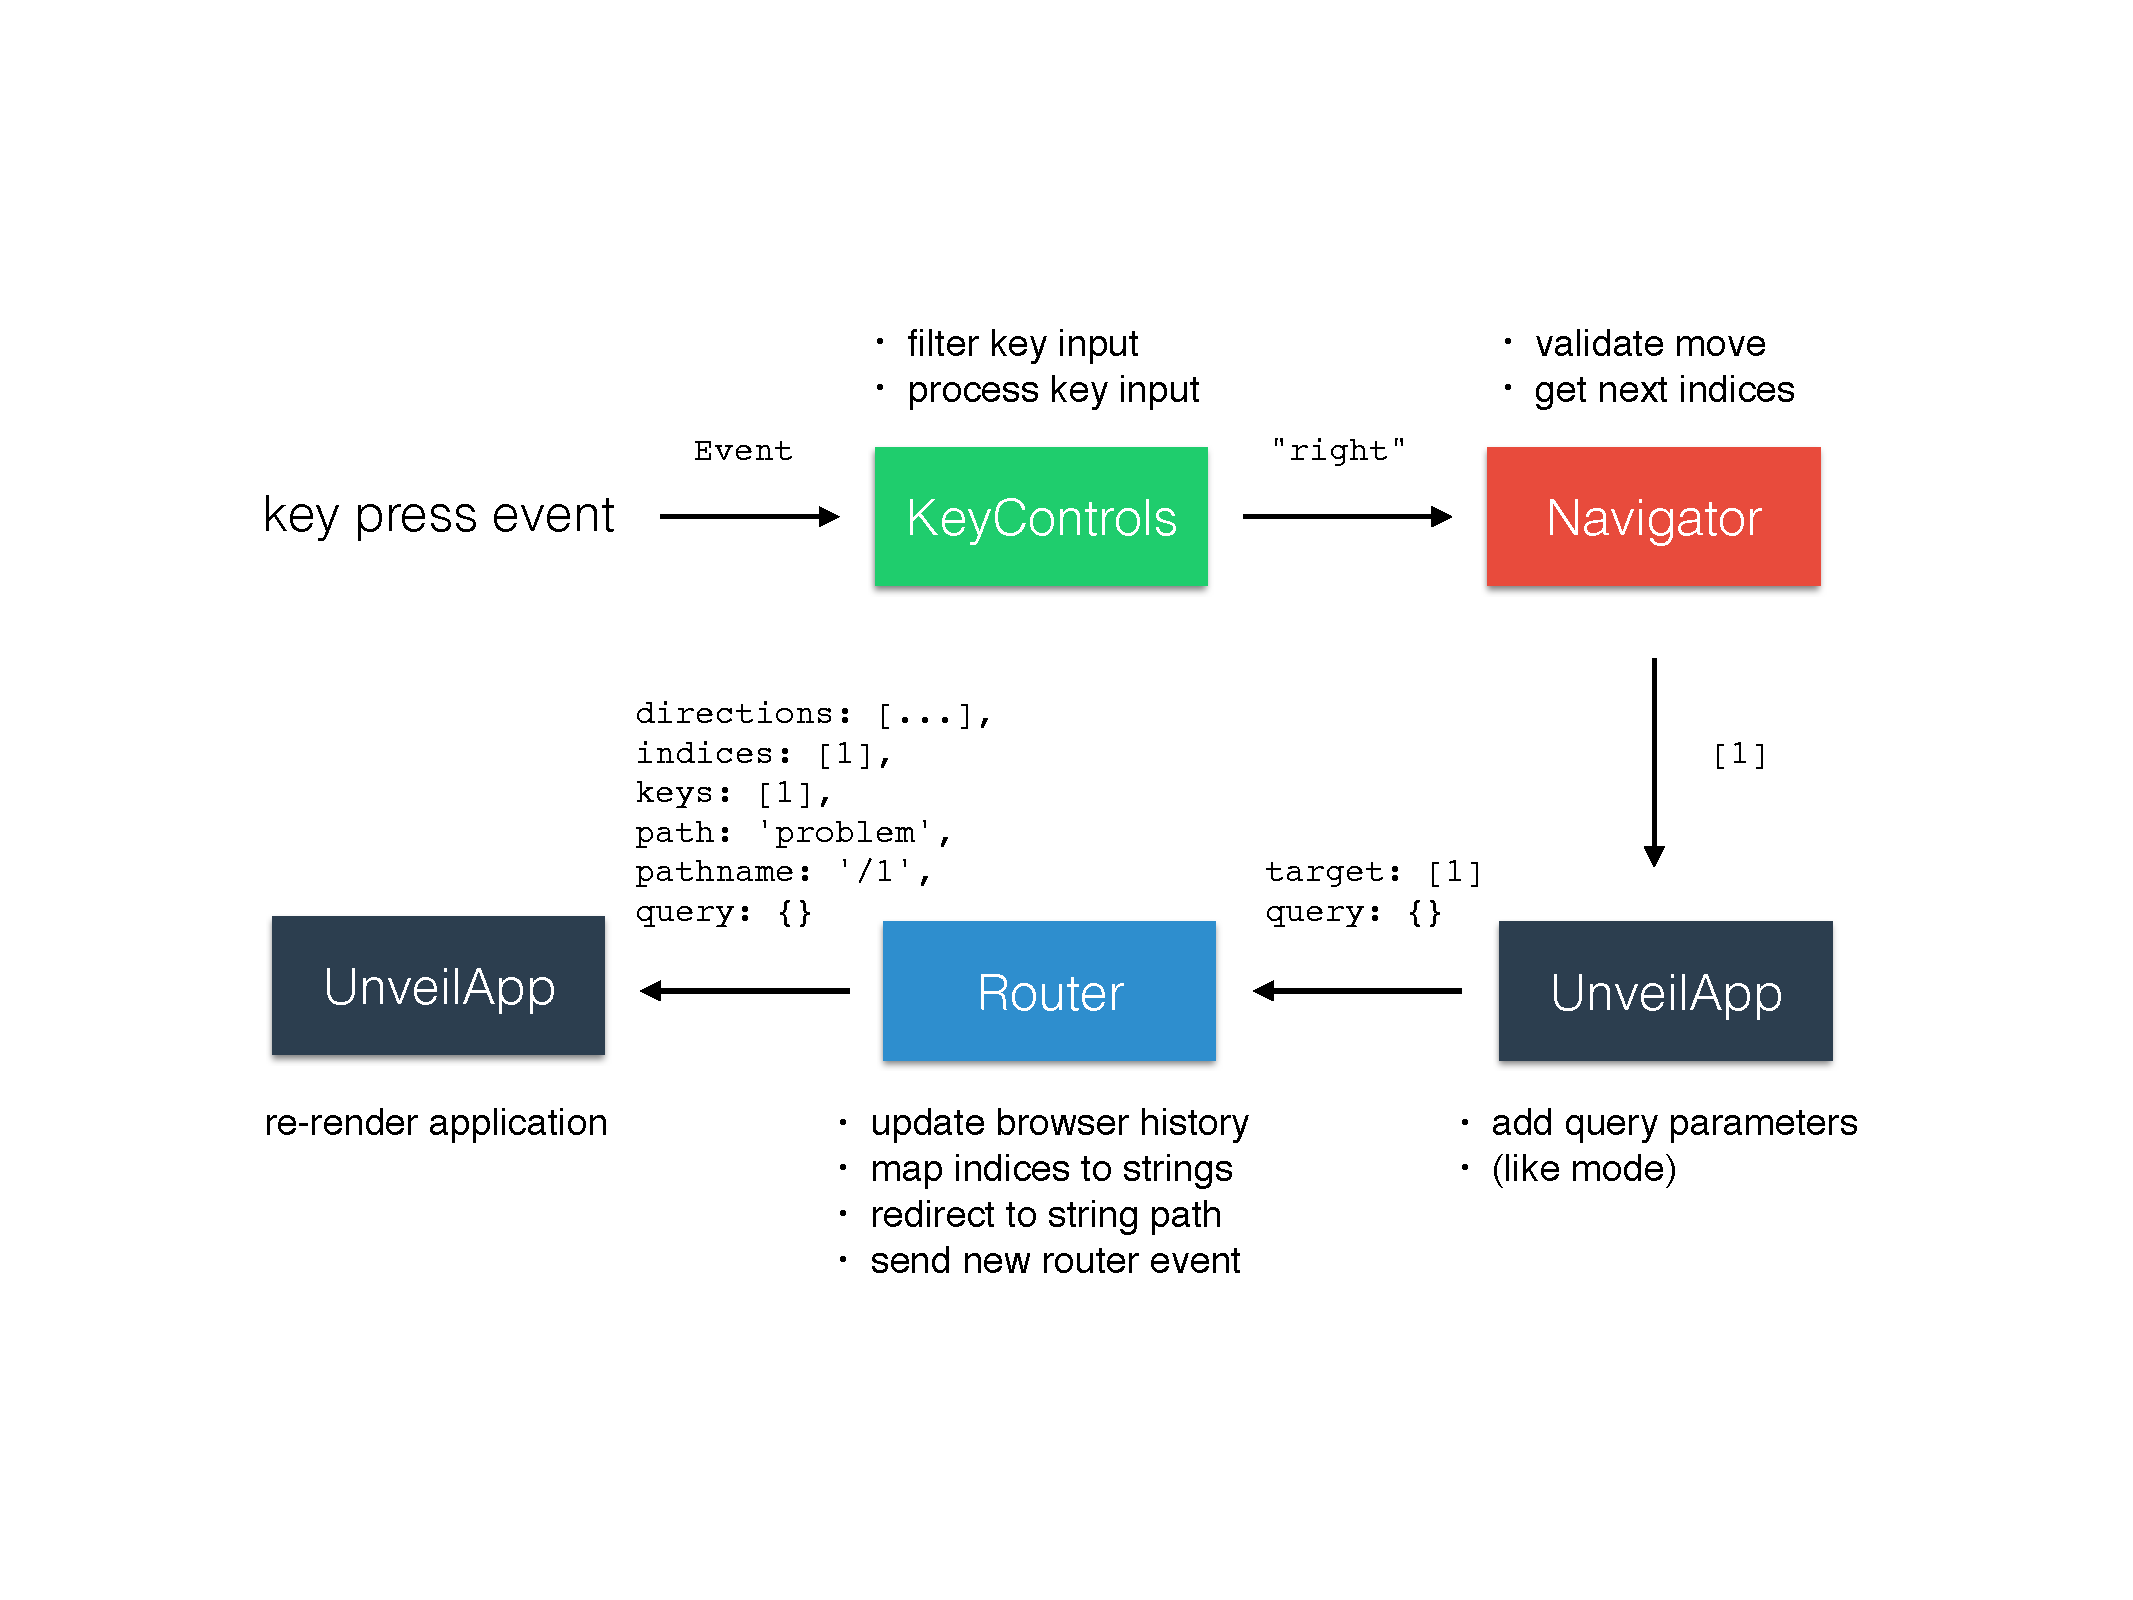
\includegraphics[width=.85\textwidth]{navigation}
\caption{Navigation pipeline from user's key press to re-render of the presentation. The monospaced text next to the arrows symbolises the data transmitted. The \texttt{KeyControls} listen for key events and process them, to then send a navigation request to go \emph{right} to the \texttt{Navigator}. This component then maps the direction to the next slide's indices (in this case $1$). \texttt{UnveilApp} then adds other information necessary for the \texttt{Router}, which then is responsible for updating the browser history, mapping the indices back to a human readable url and sending out a new router event. In the end \texttt{UnveilApp} receives this event and re-renders the presentation.}
\label{fig:implementation-technologies-unveil-navigation}
\end{figure}

%\subsection[socket.io]%
%             {socket.io%
%             \protect\footnote{\url{http://socket.io/}}}%
%\label{sec:implementation-architecture-socketio}
% problematic, talk about alternatives and problems in production, maybe even HTTP2
% e.g. safari conntection issues
% broadcasting functionality didn't quite work
% corporate firewalls can be a problem! big, in comparison to others

\section{Project Structure}
\label{sec:implementation-structure}
% A graphic explaining how the repos are built on top of each other would be great
% Which repos do I have and what do they include functionality-wise?
% explain why different repos and how they are all own npm packages that can easily be included in other projects

%\begin{figure}
%\centering
%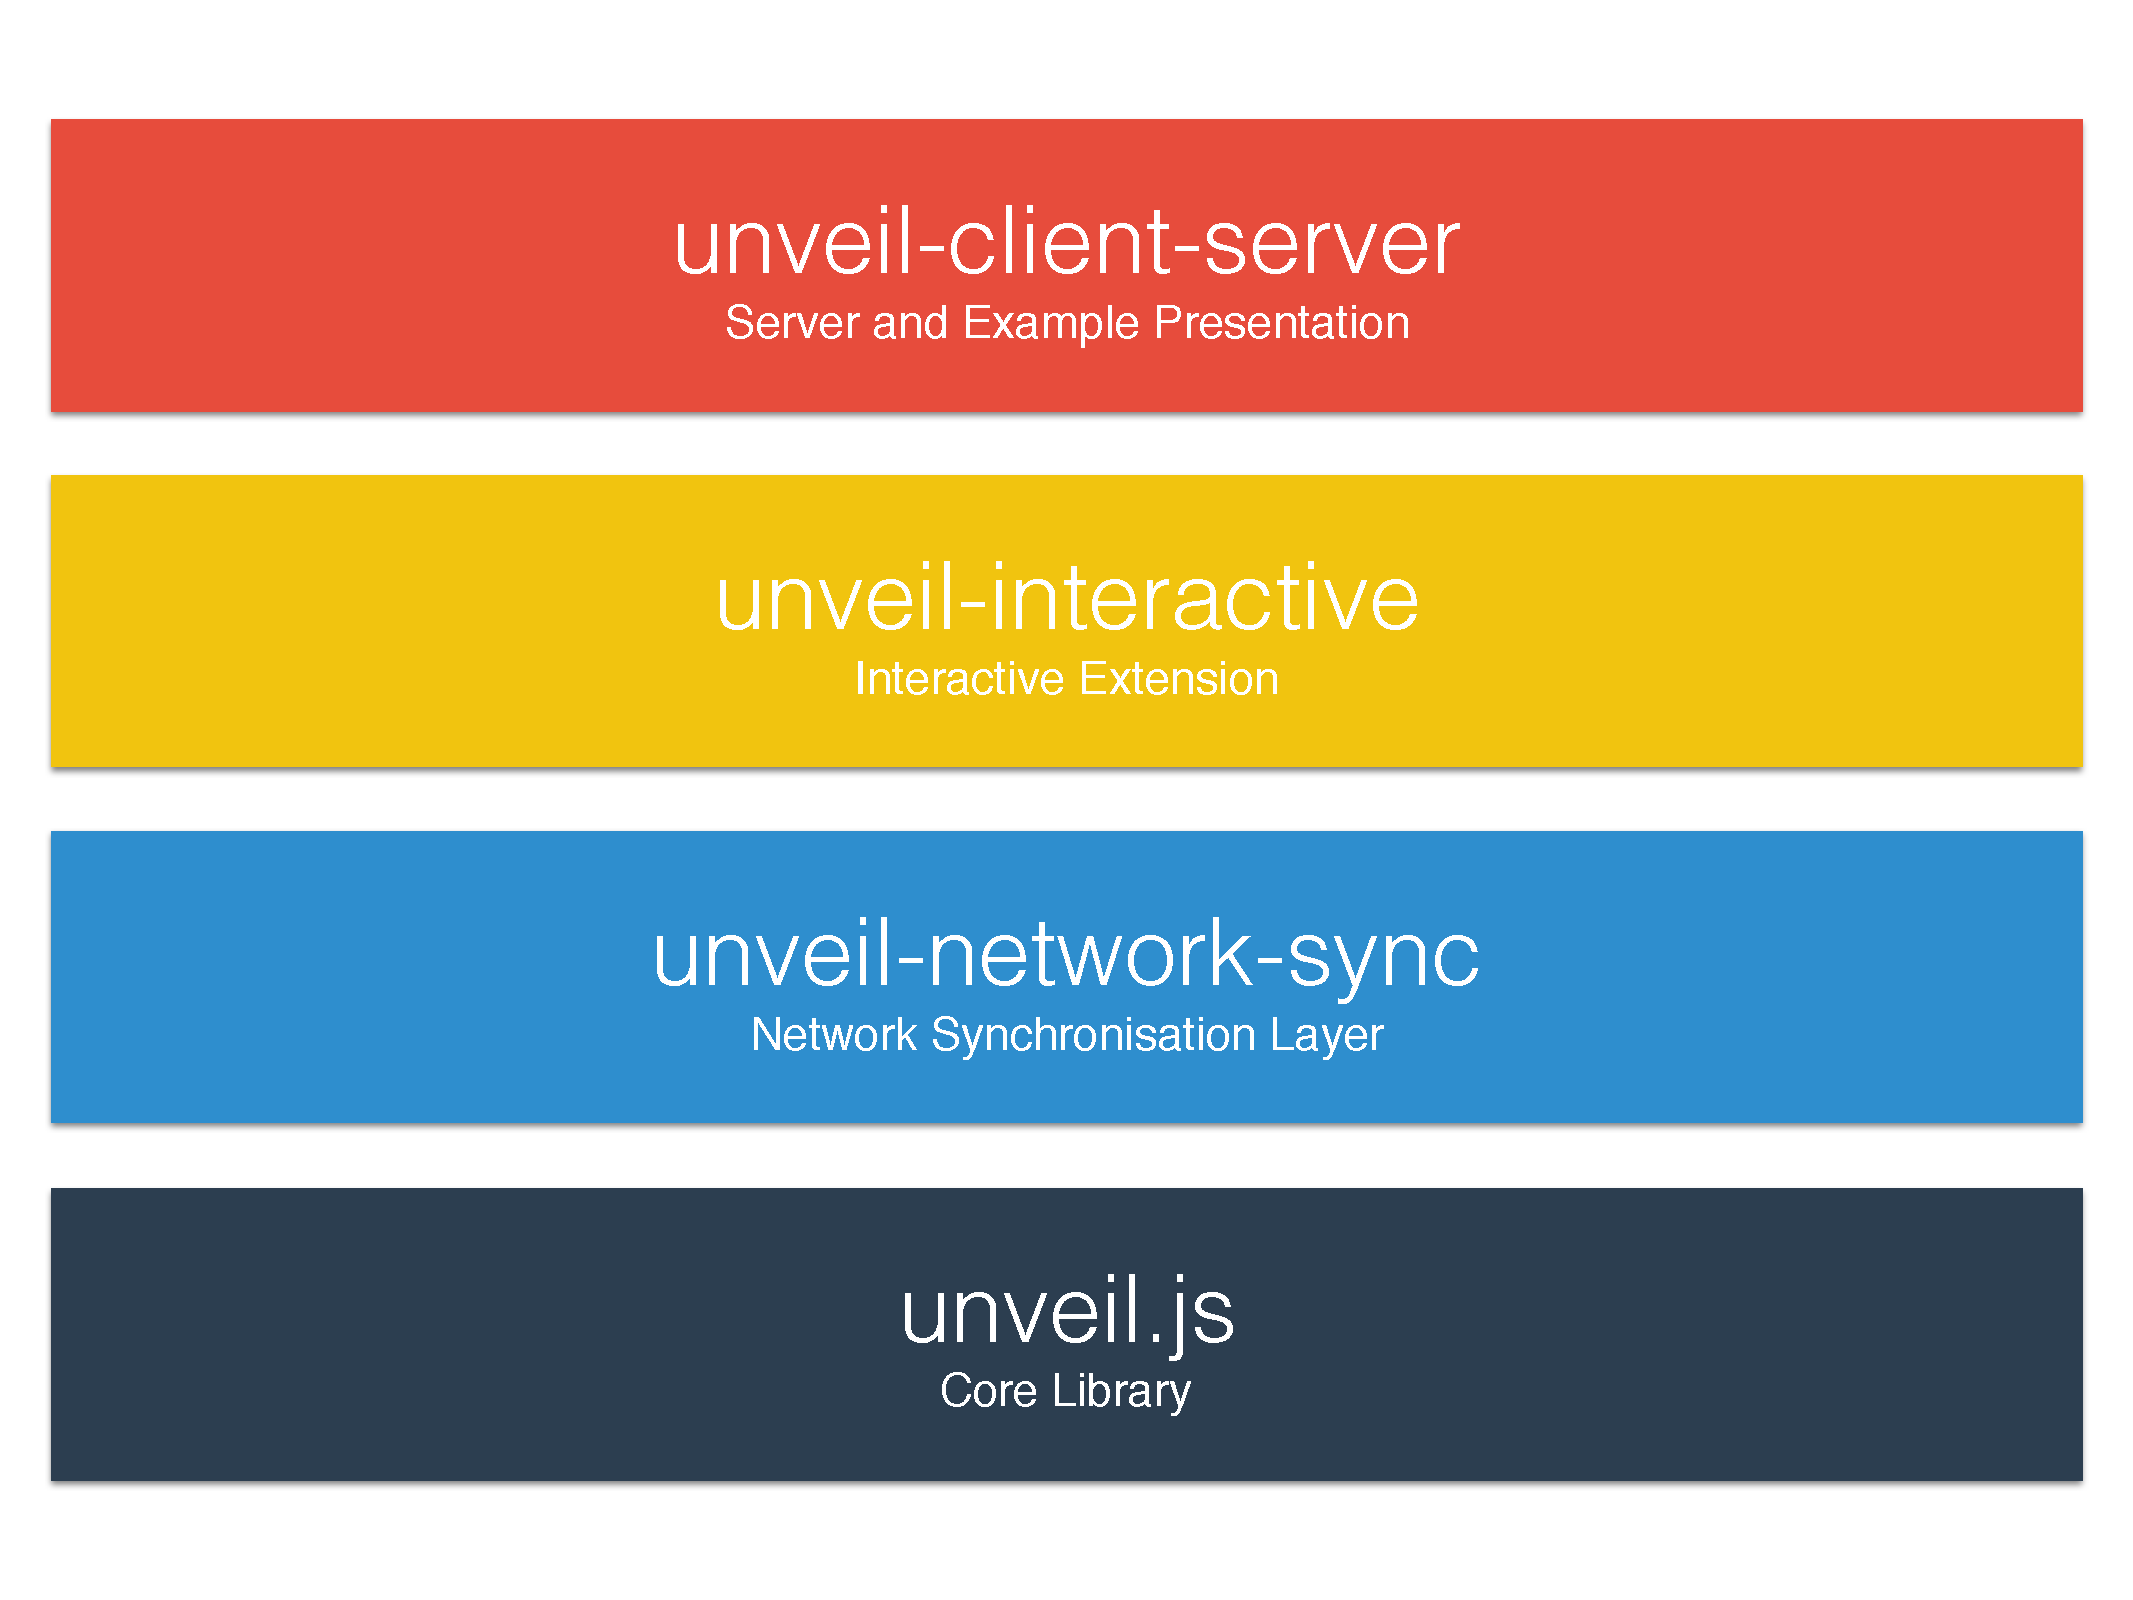
\includegraphics[width=.8\textwidth]{repos}
%\caption{Overview over GitHub repositories involved in the project. The higher ones rely on the lower ones.}
%\label{fig:implementation-structure-repos}
%\end{figure}

As the puropose of this project was not only to experiment with different ways of interacting with presentations using mobile devices, but also to create something worthwhile and contribute back to the vibrant open-source community, the project is separated into different repositories, which are all available on GitHub. These can be installed using npm, therefore allowing developers to rely only on the parts they really need.

\paragraph{Network Synchronisation Layer:} The first library of direct importance for the interaction between speaker and audience through personal devices is \textit{unveil-network-sync}\footnote{\url{https://github.com/irisSchaffer/unveil-network-sync}}. This rather small library relies on unveil.js and is responsible for connecting the client and the server through web sockets and enables the synchronisation of the current slide displayed between speaker, audience and projector. The implementation of the features will be discussed in detail in section \ref{sec:implementation-network-sync}.

\paragraph{Interactive Extension:} As the name already suggests, this library is at the core of the present thesis: It sets up a dedicated view for the speaker, implements the insertion of additional slides and subslides and by that allows for sharing of content from the audience. The voting mechanism, as well as the creation of new votings on-the-fly, also live within this library. The repository, called \emph{unveil-interactive}\footnote{\url{https://github.com/irisSchaffer/unveil-interactive}} relies on unveil-network-sync for the socket-interaction. The library will be covered in section \ref{sec:implementation-interactive} of this chapter.

\paragraph{Server and Example Presentation:} The last repository connected to this thesis is \emph{unveil-client-server}\footnote{\url{https://github.com/irisSchaffer/unveil-client-server}}, which includes a simple server as well as a real-world example of a presentation, which was used in the intermediate thesis project presentation as part of the Interactive Media course IM690, on the 2\textsuperscript{nd}\xspace of February, 2016. In this chapter, a whole section was dedicated to the server (\ref{sec:implementation-server}), as well as to the example application (\ref{sec:implementation-client}), to separate concerns a bit more clearly and be able to conclude the chapter with a demonstration of how all parts discussed earlier play together in the final presentation.

\section{Extended unveil.js}
\label{sec:implementation-unveil}

\section{Network Synchronisation Library}
\label{sec:implementation-network-sync}

\section{Interactive Library}
\label{sec:implementation-interactive}

\section{Server}
\label{sec:implementation-server}

\section{Example Application}
\label{sec:implementation-client}
% how is everything defined? what has to be included?
% what are the steps of building an application with unveil?
% how are the slides defined? how are they styled? what about the modes?
% shortly talk about server and how any server could really be used for this.